\documentclass[tikz,border=10pt]{standalone}
\usetikzlibrary{shapes.geometric, decorations.pathmorphing}

\tikzset{
    plaquette/.style={draw, fill=white, rectangle, minimum size=2cm},
    excited/.style={draw, fill=yellow, rectangle, minimum size=2cm},
    defect/.style={fill=red, circle, inner sep=2pt}
}

\begin{document}
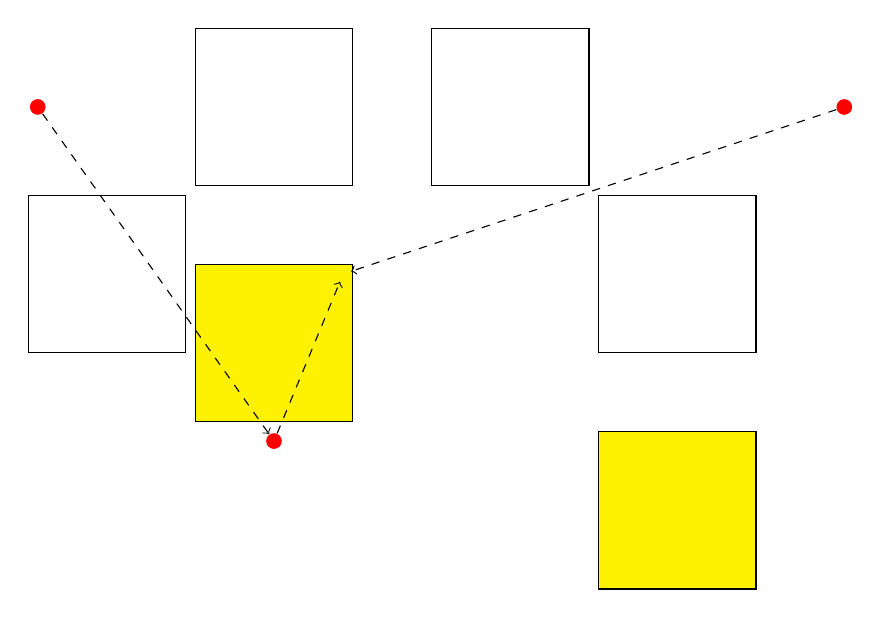
\begin{tikzpicture}[node distance=3cm]

% Ground State
\node[plaquette] (A) {};
\node[plaquette] (B) [right of=A] {};
\node[plaquette] (C) [below right of=B] {};
\node[plaquette] (D) [below left of=A] {};

% Defects
\node[defect] (Defect1) [left of=A] {};
\node[defect] (Defect2) [above right of=C] {};
\node[defect] (Defect3) [below right of=D] {};
\node[defect] (Defect4) [below left of=B] {};

% Excited Plaquettes
\node[excited] (Excited1) [below of=A] {};
\node[excited] (Excited2) [below of=C] {};

% Movement of Defects
\draw[dashed,->] (Defect1) -- (Defect3);
\draw[dashed,->] (Defect2) -- (Defect4);

% Fusing Central Two Defects
\draw[dashed,->] (Defect3) -- (Defect4);

\end{tikzpicture}
\end{document}